%%%%%%%%%%%%%%
%% Run LaTeX on this file several times to get Table of Contents,
%% cross-references, and citations.

%% If you have font problems, you may edit the w-bookps.sty file
%% to customize the font names to match those on your system.

%% w-bksamp.tex. Current Version: Feb 16, 2012
%%%%%%%%%%%%%%%%%%%%%%%%%%%%%%%%%%%%%%%%%%%%%%%%%%%%%%%%%%%%%%%%
%
%  Sample file for
%  Wiley Book Style, Design No.: SD 001B, 7x10
%  Wiley Book Style, Design No.: SD 004B, 6x9
%
%
%  Prepared by Amy Hendrickson, TeXnology Inc.
%  http://www.texnology.com
%%%%%%%%%%%%%%%%%%%%%%%%%%%%%%%%%%%%%%%%%%%%%%%%%%%%%%%%%%%%%%%%

%%%%%%%%%%%%%
% 7x10
%\documentclass{wileySev}

% 6x9
\documentclass{wileySix}

\usepackage{graphicx}

%%%%%%%
%% for times math: However, this package disables bold math (!)
%% \mathbf{x} will still work, but you will not have bold math
%% in section heads or chapter titles. If you don't use math
%% in those environments, mathptmx might be a good choice.

% \usepackage{mathptmx}

% For PostScript text
\usepackage{w-bookps}

%%%%%%%%%%%%%%%%%%%%%%%%%%%%%%%%%%%%%%%%%%%%%%%%%%%%%%%%%%%%%%%%
%% Other packages you might want to use:

% for chapter bibliography made with BibTeX
% \usepackage{chapterbib}

% for multiple indices
% \usepackage{multind}

% for answers to problems
% \usepackage{answers}

%%%%%%%%%%%%%%%%%%%%%%%%%%%%%%
%% Change options here if you want:
%%
%% How many levels of section head would you like numbered?
%% 0= no section numbers, 1= section, 2= subsection, 3= subsubsection
%%==>>
\setcounter{secnumdepth}{3}

%% How many levels of section head would you like to appear in the
%% Table of Contents?
%% 0= chapter titles, 1= section titles, 2= subsection titles, 
%% 3= subsubsection titles.
%%==>>
\setcounter{tocdepth}{2}

%% Cropmarks? good for final page makeup
%% \docropmarks

%%%%%%%%%%%%%%%%%%%%%%%%%%%%%%
%
% DRAFT
%
% Uncomment to get double spacing between lines, current date and time
% printed at bottom of page.
% \draft
% (If you want to keep tables from becoming double spaced also uncomment
% this):
% \renewcommand{\arraystretch}{0.6}
%%%%%%%%%%%%%%%%%%%%%%%%%%%%%%

%%%%%%% Demo of section head containing sample macro:
%% To get a macro to expand correctly in a section head, with upper and
%% lower case math, put the definition and set the box 
%% before \begin{document}, so that when it appears in the 
%% table of contents it will also work:

\newcommand{\VT}[1]{\ensuremath{{V_{T#1}}}}

%% use a box to expand the macro before we put it into the section head:

\newbox\sectsavebox
\setbox\sectsavebox=\hbox{\boldmath\VT{xyz}}

%%%%%%%%%%%%%%%%% End Demo


\begin{document}


\booktitle{Survey Methodology}
\subtitle{This is the Subtitle}

\authors{Robert M. Groves\\
\affil{Universitat de les Illes Balears}
Floyd J. Fowler, Jr.\\
\affil{University of New Mexico}
}

\offprintinfo{Survey Methodology, Second Edition}{Robert M. Groves}

%% Can use \\ if title, and edition are too wide, ie,
%% \offprintinfo{Survey Methodology,\\ Second Edition}{Robert M. Groves}

%%%%%%%%%%%%%%%%%%%%%%%%%%%%%%
%% 
\halftitlepage

\titlepage


\begin{copyrightpage}{2007}
Survey Methodology / Robert M. Groves . . . [et al.].
\       p. cm.---(Wiley series in survey methodology)
\    ``Wiley-Interscience."
\    Includes bibliographical references and index.
\    ISBN 0-471-48348-6 (pbk.)
\    1. Surveys---Methodology.  2. Social 
\  sciences---Research---Statistical methods.  I. Groves, Robert M.  II. %
Series.\\

HA31.2.S873 2007
001.4'33---dc22                                             2004044064
\end{copyrightpage}



\dedication{To my parents}

\begin{contributors}
\name{Masayki Abe,} Fujitsu Laboratories Ltd., Fujitsu Limited, Atsugi,
Japan

\name{L. A. Akers,} Center for Solid State Electronics Research, Arizona
State University, Tempe, Arizona

\name{G. H. Bernstein,} Department of Electrical and
Computer Engineering, University of Notre Dame, Notre Dame, South Bend, 
Indiana; formerly of
Center for Solid State Electronics Research, Arizona
State University, Tempe, Arizona 
\end{contributors}

\contentsinbrief
\tableofcontents
\listoffigures
\listoftables


\begin{foreword}
This is the foreword to the book.
\end{foreword}

\begin{preface}
This is an example preface.
This is an example preface.
This is an example preface.
This is an example preface.

\prefaceauthor{R. K. Watts}
\where{Durham, North Carolina\\
September, 2007}

\end{preface}


\begin{acknowledgments}
From Dr.~Jay Young, consultant from Silver Spring, Maryland, I received
the initial push to even consider writing this book. Jay was a constant
``peer reader'' and very welcome advisor durying this year-long process.


To all these wonderful people I owe a deep sense of gratitude especially now
that this project has been completed.
\authorinitials{G. T. S.}
\end{acknowledgments}

\begin{acronyms}
\acro{ACGIH}{American Conference of Governmental Industrial Hygienists}
\acro{AEC}{Atomic Energy Commission}
\acro{OSHA}{Occupational Health and Safety Commission}
\acro{SAMA}{Scientific Apparatus Makers Association}
\end{acronyms}

\begin{glossary}
\term{NormGibbs}Draw a sample from a posterior distribution
of data with an unknown mean and variance using Gibbs sampling.

\term{pNull}Test a one sided hypothesis from a numberically
specified posterior CDF or from a sample from the posterior

\term{sintegral}A numerical integration using Simpson's rule
\end{glossary}

\begin{symbols}
\term{A}Amplitude

\term{\hbox{\&}}Propositional logic symbol 

\term{a}Filter Coefficient

\bigskip

\term{\mathcal{B}}Number of Beats
\end{symbols}

\begin{introduction}

%% optional, but if you want to list author:

\introauthor{Catherine Clark, PhD.}
{Harvard School of Public Health\\
Boston, MA, USA}

The era of modern \index{microelectronics}\index{microelectronics!modern} 
began in 1958 with the invention of the
integrated circuit by J.~S.~Kilby
 of Texas Instruments \cite{kilby}.
His first chip is shown in Fig.~I. For comparison,
Fig.~I.2 shows a modern microprocessor chip, \cite{beren}.


This is the introduction.
This is the introduction.
This is the introduction.
This is the introduction.
This is the introduction.
This is the introduction.

\begin{equation}
ABC {\cal DEF} \alpha\beta\Gamma\Delta\sum^{abc}_{def}
\end{equation}


\begin{chapreferences}{3.}
\bibitem{zkilby}J. S. Kilby,
``Invention of the Integrated Circuit,'' {\it IEEE Trans. Electron Devices,}
{\bf ED-23,} 648 (1976).

\bibitem{zhamming}R. W. Hamming,
                 {\it Numerical Methods for Scientists and 
                 Engineers}, Chapter N-1, McGraw-Hill, 
                 New York, 1962.

\bibitem{zHu}J. Lee, K. Mayaram, and C. Hu, ``A Theoretical
               Study of Gate/Drain Offset in LDD MOSFETs''
                     {\it IEEE Electron Device Lett.,} {\bf EDL-7}(3). 152 
                     (1986).
\end{chapreferences}
\end{introduction}

\chapter{Installation}

\chapter{Your First Document}

\chapter{Structuring Your Document (Section and Paragraph)}
\section{Structuring Your Document}

\hspace{0.50in} Membuat dokumen yang sangat mendasar telah kita pelajari dalam materi sebelumnya, namun saat menulis makalah Anda perlu menyusun konten ke dalam unit logika. Untuk mencapai hal ini, LaTeX menawarkan perintah untuk menghasilkan judul bagian dan mencatatnya secara otomatis. Perintah untuk membuat judul bagian sangat mudah: \par
{\fontsize{10pt}{10pt}\selectfont  $  \setminus  $section $  \{  $ $  \}  $}
 \par
{\fontsize{10pt}{10pt}\selectfont  $  \setminus  $subsection $  \{  $ $  \}  $}
 \par
{\fontsize{10pt}{10pt}\selectfont  $  \setminus  $subsubsection $  \{  $ $  \}  $}
 \par
{\fontsize{10pt}{10pt}\selectfont  $  \setminus  $paragraph $  \{  $ $  \}  $}
 \par
{\fontsize{10pt}{10pt}\selectfont  $  \setminus  $subparagraph $  \{  $ $  \}  $}
 \par

Hasil \ref{dokumen} Dokumen:
\begin{figure}[ht]
	\centerline{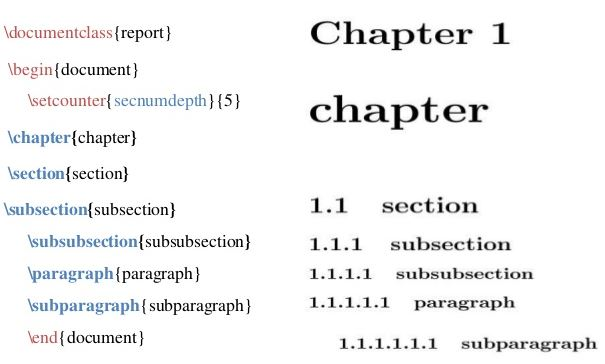
\includegraphics[width=0.50\textwidth]{gambar/dokumen}}
	\caption{dokumen}
	\label{dokumen}
\end{figure}

\vspace{50pt}
\hspace{0.50in} Sedangkan dokumen kelas report dan book selain memiliki perintah-perintah di atas memiliki juga perintah :
 \par
{\fontsize{10pt}{10pt}\selectfont  $  \setminus  $part $  \{  $... $  \}  $}
 \par
\vspace{9pt}

{\fontsize{10pt}{10pt}\selectfont  $  \setminus  $chapter $  \{  $... $  \}  $}
 \par
\vspace{9pt}
{\fontsize{10pt}{10pt}\selectfont  $  \setminus  $frontmatter}
 \par
\vspace{9pt}
{\fontsize{10pt}{10pt}\selectfont  $  \setminus  $mainmatter}
 \par
\vspace{9pt}
{\fontsize{10pt}{10pt}\selectfont  $  \setminus  $backmatter}
 \par
\vspace{12pt}
\hspace{0.50in} Argumen yang diberikan pada perintah-perintah ini adalah nama bab, subbab, dll. Dalam naskah buku yang dituliskan dengan kelas dokumen book, fronmatter digunakan untuk menandai halaman judul, daftar isi, kata pengantar, daftar gambar, dsb. Sedangkan mainmatter digunakan untuk menandai bagian tulisan utama, dan backmatter untuk menandai daftar pustaka, indeks, daftar istilah, dsb. Perintah  $  \setminus  $chapter,  $  \setminus  $section,  $  \setminus  $subsection, dan  $  \setminus  $subsubsection secara otomatis memberikan nomor pada nama bagian, bab, dsb. Jika nomor ini tidak diinginkan, perintah yang ekivalen adalah  $  \setminus  $chapter*,  $  \setminus  $section*,  $  \setminus  $subsection*, dan  $  \setminus  $subsubsection*.
 \par
\vspace{12pt}
\hspace{0.50in} Perintah bagian diberi nomor dan akan muncul dalam daftar isi dokumen. Paragraf tidak diberi nomor dan tidak akan ditampilkan dalam daftar isi. Berikut contoh output menggunakan bagian:
 \par
1 Section
 \par
~~ Hello World!
 \par
~~~~~ 1.1 Subsection
 \par
~~~~~~~~~~~~ Structuring a document is easy
 \par
\vspace{12pt}
\hspace{0.50in} Untuk mendapatkan hasil ini, Anda hanya perlu menambahkan beberapa baris ke program kami dari pelajaran 1:
 \par
 $  \setminus  $documentclass $  \{  $article $  \}  $
 \par
\vspace{12pt}
 $  \setminus  $title $  \{  $Title of my document $  \}  $
 \par
 $  \setminus  $date $  \{  $2013-09-01 $  \}  $
 \par
 $  \setminus  $author $  \{  $John Doe $  \}  $
 \par
\vspace{12pt}
 $  \setminus  $begin $  \{  $document $  \}  $
 \par
\vspace{12pt}
 $  \setminus  $maketitle
 \par
 $  \setminus  $pagenumbering $  \{  $gobble $  \}  $
 \par

 $  \setminus  $newpage
 \par
 $  \setminus  $pagenumbering $  \{  $arabic $  \}  $
 \par
\vspace{12pt}
 $  \setminus  $section $  \{  $Section $  \}  $
 \par
\vspace{12pt}
Hello World!
 \par
\vspace{12pt}
 $  \setminus  $subsection $  \{  $Subsection $  \}  $
 \par
\vspace{12pt}
Structuring a document is easy!
 \par
\vspace{12pt}
 $  \setminus  $end $  \{  $document $  \}  $
 \par
\vspace{14pt}
Gambar berikut menunjukkan struktur hirarkis dari semua elemen:
 \par
1. Section
 \par
~~~ Hello World
 \par
~~~~ 1.1 Subsection
 \par
~~~~~~~~~~ Structuring a document is easy!
 \par
~~~~~~~~~ 1.1 Subsection
 \par
~~~~~~~~~~~~~~~ More Text
 \par
~~~~~~~~~~~~~~~ Paragraph ~~~~~~~~~~~~ Some more text
 \par
~~~~~~~~~~~~~~~ Subparagraph ~~~~~~~ Even more text \par
2. Another Section
 \par
\hspace{0.50in} Saya telah menggunakan kode berikut untuk mendapatkan output ini:
 \par
 $  \setminus  $documentclass $  \{  $article $  \}  $
 \par
\vspace{12pt}
 $  \setminus  $begin $  \{  $document $  \}  $
 \par
\vspace{12pt}
 $  \setminus  $section $  \{  $Section $  \}  $
 \par
\vspace{12pt}
Hello World!
 \par
\vspace{12pt}
 $  \setminus  $subsection $  \{  $Subsection $  \}  $
 \par
\vspace{12pt}
Structuring a document is easy!
 \par
\vspace{12pt}
 $  \setminus  $subsubsection $  \{  $Subsubsection $  \}  $
 \par
\vspace{12pt}
More text.
 \par
\vspace{12pt}
 $  \setminus  $paragraph $  \{  $Paragraph $  \}  $
 \par
\vspace{12pt}
Some more text.
 \par
\vspace{12pt}
 $  \setminus  $subparagraph $  \{  $Subparagraph $  \}  $
 \par
\vspace{12pt}
Even more text.
 \par
\vspace{12pt}
 $  \setminus  $section $  \{  $Another section $  \}  $
 \par
\vspace{12pt}
 $  \setminus  $end $  \{  $document $  \}  $
 \par
\vspace{12pt}
\vspace{12pt}
Contoh struktur dokumen berkelas article dan book :
 \par
{\fontsize{10pt}{10pt}\selectfont  $  \setminus  $documentclass $  \{  $article $  \}  $}
 \par
\vspace{10pt}
{\fontsize{10pt}{10pt}\selectfont  $  \setminus  $usepackage $  \{  $... $  \}  $}
 \par
\vspace{10pt}
{\fontsize{10pt}{10pt}\selectfont  $  \setminus  $begin $  \{  $document $  \}  $}
 \par
\vspace{10pt}
{\fontsize{10pt}{10pt}\selectfont  $  \setminus  $maketitle}
 \par
\vspace{10pt}
{\fontsize{10pt}{10pt}\selectfont  $  \setminus  $section $  \{  $... $  \}  $}
 \par
\vspace{10pt}
{\fontsize{10pt}{10pt}\selectfont  $  \setminus  $section $  \{  $... $  \}  $}
 \par
\vspace{10pt}
{\fontsize{10pt}{10pt}\selectfont  $  \setminus  $subsection $  \{  $... $  \}  $}
 \par
\vspace{10pt}
{\fontsize{10pt}{10pt}\selectfont  $  \setminus  $subsubsection $  \{  $... $  \}  $}
 \par
\vspace{10pt}
{\fontsize{10pt}{10pt}\selectfont  $  \setminus  $section}
 \par
\vspace{10pt}
{\fontsize{10pt}{10pt}\selectfont  $  \setminus  $end $  \{  $document $  \}  $}
 \par
\vspace{12pt}
\hspace{0.50in} LaTeX dapat menyusun dokumen menjadi beberapa bagian dengan sangat mudah. Hal ini karena LaTeX memiliki format yang konsisten di seluruh kertas. Berikut perintah-perintah latex, seperti:
 \begin{itemize}
\item part \par
\textit{part} berfungsi untuk membuat pembagian bab, biasanya dibuat dalam halaman yang terpisah. Adapun penggunaannya adalah sebagai berikut:

{\fontsize{10pt}{10pt}\selectfont ~~  $  \setminus  $part $  \{  $[Judul] $  \}  $}
 \par
\item chapter \par
\textit{chapter} merupakan bab utama yang memuat judul. Penggunaannya demikian:
\par
{\fontsize{10pt}{10pt}\selectfont ~~  $  \setminus  $chapter $  \{  $[Judul] $  \}  $}
\par
\item section \par
\textit{section} merupakan pasal dari suatu bab. Contoh penggunaannya adalah sebagai berikut:\
 \par
{\fontsize{10pt}{10pt}\selectfont ~~~  $  \setminus  $section $  \{  $[Judul] $  \}  $}
 \par
\item subsection \par
subsection \textit{subsection} berfungsi untuk membuat sub pasal atau pasal baru di bawah judul pasal.
 \par
{\fontsize{10pt}{10pt}\selectfont ~~  $  \setminus  $subsection $  \{  $Judul $  \}  $}
 \par
\textit{subsubsection} berfungsi untuk membuat sub pasal di bawahnya lagi dari sub pasal yang ada.
 \par
{\fontsize{10pt}{10pt}\selectfont ~~  $  \setminus  $subsubsection* $  \{  $Judul $  \}  $}
 \par
 \item paragraph \par
\textit{paragraph} berguna untuk membuat alinea kalimat, cara penggunaannya adalah sebagai berikut:
 \par
{\fontsize{10pt}{10pt}\selectfont ~~  $  \setminus  $paragraph $  \{  $kalimat $  \}  $}
 \par
\item subparagraph \par
\textit{subpragraph} berfungsi untuk membuat alinea baru di dalam alinea yang sudah ada. Cara penggunaannya adalah demikian:
 \par
{\fontsize{10pt}{10pt}\selectfont ~~  $  \setminus  $subparagraph $  \{  $kalimat $  \}  $}
 \par
 \vspace{12pt}
Contoh struktur dokumen berikut ini:
 \par
{\fontsize{10pt}{10pt}\selectfont  $  \setminus  $part $  \{  $Memulai LATEX $  \}  $  $  \%  $ ini adalah contoh penggunaan part}
 \par
{\fontsize{10pt}{10pt}\selectfont ~~~~~  $  \setminus  $chapter $  \{  $Menggunakan LATEX $  \}  $  $  \%  $ ini adalah contoh penggunaan chapter}
 \par
{\fontsize{10pt}{10pt}\selectfont ~~~~~~~~~~~  $  \setminus  $section $  \{  $Penggunaan Class dalam penulisan dokumen $  \}  $}
 \par
{\fontsize{10pt}{10pt}\selectfont  \hspace*{0.64in} ~  \hspace*{0.64in}  \hspace*{0.64in}  $  \%  $ ini adalah contoh penggunaan section}
 \par
{\fontsize{10pt}{10pt}\selectfont ~~~~~~~~~~~~~~~~ $  \setminus  $subsection $  \{  $Penyertaan Package $  \}  $  }
 \par
{\fontsize{10pt}{10pt}\selectfont  \hspace*{0.64in}  \hspace*{0.64in}  \hspace*{0.64in}  $  \%  $ ini adalah contoh penggunaan subsection}
 \par
{\fontsize{10pt}{10pt}\selectfont  \hspace*{0.64in}  \hspace*{0.64in}  \hspace*{0.64in}  $  \setminus  $paragraph $  \{  $Penyertaan package berguna untuk menambahkan fungsi }
 \par
{\fontsize{10pt}{10pt}\selectfont  \hspace*{0.64in}  \hspace*{0.64in}  \hspace*{0.64in} kedalam dokumen/naskah yang kita buat. Bentuk penulisannya }
 \par
{\fontsize{10pt}{10pt}\selectfont  \hspace*{0.64in}  \hspace*{0.64in}  \hspace*{0.64in} adalah sebagai berikut: $  \}  $}
 \par
{\fontsize{10pt}{10pt}\selectfont   \hspace*{0.64in}  \hspace*{0.64in}  \hspace*{0.64in}  \hspace*{0.64in}  $  \%  $ ini adalah contoh penggunaan paragraph}
 \par
\end{itemize}
\vspace{10pt}
\subsection{Komentar}
 \par
\hspace{0.50in} Fungsi dari komentar adalah untuk menampilkan catatan dari naskah yang telah Anda buat, namun tidak ditampilkan pada saat file dicetak. Contoh penggunaan nya adalah sebagai berikut:
 \par
{\fontsize{10pt}{10pt}\selectfont  $  \setminus  $documentclass[12pt,a4paper,oneside,bahasa,dvips] $  \{  $book $  \}  $}
 \par
{\fontsize{10pt}{10pt}\selectfont  $  \setminus  $begin $  \{  $document $  \}  $}
 \par
{\fontsize{10pt}{10pt}\selectfont Halo, ini adalah contoh penulisan menggunakan LaTeX.}
 \par
{\fontsize{10pt}{10pt}\selectfont ukuran font dari naskah ini adalah 12. Pencetakan akan menggunakan}
 \par
{\fontsize{10pt}{10pt}\selectfont kertas A4, yang akan dicetak dalam satu sisi. Naskah ini berbentuk bu}
 \par
{\fontsize{10pt}{10pt}\selectfont dan akan ditampilkan kedalam bahasa Indonesia.}
 \par
{\fontsize{10pt}{10pt}\selectfont komentar ini tidak akan ditampilkan pada saat dilakukan pencetakan}
 \par
{\fontsize{10pt}{10pt}\selectfont naskah.}
 \par
{\fontsize{10pt}{10pt}\selectfont  $  \setminus  $end $  \{  $document $  \}  $}
 \par
\subsection{Membuat Judul Dokumen}
 \par
Untuk judul dokumen, perintahnya adalah sebagai berikut:
 \par
{\fontsize{10pt}{10pt}\selectfont  $  \setminus  $title $  \{  $ $  \}  $}
 \par
{\fontsize{10pt}{10pt}\selectfont  $  \setminus  $maketitle}
 \par
\vspace{12pt}
Adapun contohnya adalah sebagai berikut:
 \par
{\fontsize{10pt}{10pt}\selectfont  $  \setminus  $documentclass[12pt,a4paper,oneside,bahasa,dvips] $  \{  $book $  \}  $}
 \par
{\fontsize{10pt}{10pt}\selectfont  $  \setminus  $title $  \{  $Membuat Dokumen dengan  $  \setminus  $LaTeX $  \{  $ $  \}  $ $  \}  $}
 \par
{\fontsize{10pt}{10pt}\selectfont  $  \setminus  $begin $  \{  $document $  \}  $}
 \par
{\fontsize{10pt}{10pt}\selectfont  $  \setminus  $maketitle}
 \par
\vspace{10pt}
{\fontsize{10pt}{10pt}\selectfont Halo, ini adalah contoh penulisan menggunakan LaTeX, dengan ukuran font Pencetakan akan menggunakan kertas A4, yang akan dicetak dalam satu sis Naskah ini berbentuk buku dan akan ditampilkan kedalam bahasa Indonesia judul akan ditampilkan secara otomatis pada awal dokumen ketika dokumen dikonversi ke format DVI,HTML, ataupun PDF.  $  \setminus  $end $  \{  $document $  \}  $} 

\subsection{Memisahkan Baris} \par
Untuk memisahkan baris, Anda bisa menggunakan perintah sebagai berikut: \par
 $  \setminus  $ $  \setminus  $ \par
atau \par
{\fontsize{10pt}{10pt}\selectfont  $  \setminus  $newline} \par
\vspace{12pt}
Adapun contoh penggunaannya adalah demikian: \par
Contoh 1: \par
{\fontsize{10pt}{10pt}\selectfont  $  \setminus  $documentclass[12pt,a4paper,oneside,bahasa,dvips] $  \{  $book $  \}  $} \par
{\fontsize{10pt}{10pt}\selectfont  $  \setminus  $begin $  \{  $document $  \}  $} \par
\vspace{10pt}
{\fontsize{10pt}{10pt}\selectfont Halo, ini adalah contoh penulisan menggunakan LaTeX, dengan ukuran font Pencetakan akan menggunakan kertas A4, yang akan dicetak dalam satu sis Naskah ini berbentuk buku dan akan ditampilkan kedalam bahasa Indonesia} \par
\vspace{10pt}
{\fontsize{10pt}{10pt}\selectfont Tulisan ini akan ditampilkan dengan penambahan satu baris.} \par
{\fontsize{10pt}{10pt}\selectfont  $  \setminus  $end $  \{  $document $  \}  $} \par
\vspace{10pt}
Contoh 2: \par
{\fontsize{10pt}{10pt}\selectfont  $  \setminus  $documentclass[12pt,a4paper,oneside,bahasa,dvips] $  \{  $book $  \}  $} \par
{\fontsize{10pt}{10pt}\selectfont  $  \setminus  $begin $  \{  $document $  \}  $} \par
\vspace{10pt}
{\fontsize{10pt}{10pt}\selectfont Halo, ini adalah contoh penulisan menggunakan LaTeX, dengan ukuran font Pencetakan akan menggunakan kertas A4, yang akan dicetak dalam satu sis Naskah ini berbentuk buku dan akan ditampilkan kedalam bahasa Indonesia} \par
\vspace{10pt}
{\fontsize{10pt}{10pt}\selectfont  $  \setminus  $linebreak} \par
{\fontsize{10pt}{10pt}\selectfont Tulisan ini akan ditampilkan dengan penambahan satu baris.} \par

{\fontsize{10pt}{10pt}\selectfont  $  \setminus  $end $  \{  $document $  \}  $}
 \par

\subsection{Berpindah Halaman}
 \par
Untuk berpindah halaman, Anda bisa menggunakan perintah sebagai berikut: \par
\begin{equation}
newpage
\end{equation}

\vspace{9pt}
Contohnya adalah sebagai berikut \par
{\fontsize{10pt}{10pt}\selectfont  $  \setminus  $documentclass[12pt,a4paper,oneside,bahasa,dvips] $  \{  $book $  \}  $} \par
{\fontsize{10pt}{10pt}\selectfont  $  \setminus  $title $  \{  $Membuat Dokumen dengan  $  \setminus  $LaTeX $  \{  $ $  \}  $ $  \}  $} \par
{\fontsize{10pt}{10pt}\selectfont  $  \setminus  $author $  \{  $R. Kresno Aji (masaji@ai.co.id) $  \}  $} \par
{\fontsize{10pt}{10pt}\selectfont  $  \setminus  $date $  \{  $17 Agustus 2004 $  \}  $} \par
{\fontsize{10pt}{10pt}\selectfont  $  \setminus  $begin $  \{  $document $  \}  $} \par
{\fontsize{10pt}{10pt}\selectfont  $  \setminus  $maketitle} \par
\vspace{10pt}
{\fontsize{10pt}{10pt}\selectfont Halo, ini adalah contoh penulisan menggunakan LaTeX, dengan ukuran font Pencetakan akan menggunakan kertas A4, yang akan dicetak dalam satu sis Naskah ini berbentuk buku dan akan ditampilkan kedalam bahasa Indonesia judul akan ditampilkan secara otomatis pada awal dokumen ketika dokumen dikonversi ke format DVI,HTML, ataupun PDF.} \par
\vspace{10pt}
{\fontsize{10pt}{10pt}\selectfont  $  \setminus  $newpage} \par
{\fontsize{10pt}{10pt}\selectfont  $  \setminus  $chapter $  \{  $Halaman Baru $  \}  $} \par
{\fontsize{10pt}{10pt}\selectfont  $  \setminus  $end $  \{  $document $  \}  $} \par

\subsection{Environtment} \par
LATEX menyediakan environmen yang berupa: \par
* Itemize \par
~~ berfungsi untuk membuat daftar yang tidak memiliki urutan. \par
* Enumerate \par
~~ berfungsi untuk membuat daftar yang berurutan. \par
* Flushleft \par
~~ untuk membuat kalimat rata kiri. \par
* Center \par
~~ berfungsi untuk membuat kalimat dengan format center. \par
* Flushright \par
~~ berfungsi untuk membuat kalimat rata kanan. \par
* Footnote \par
~~ berfungsi untuk membuat catatan kaki. \par
* Verbatim \par
~~ berfungsi untuk membuat kalimat / karakter yang ditulis \par
* Table
 \par
~~ berfungsi untuk membuat tabel.  \par 
\begin{enumerate}
\item  Pembuatan daftar berurutan \par
Untuk membuat daftar yang berurutan, Anda bisa menggunakan perintah berikut ini: \par
{\fontsize{10pt}{10pt}\selectfont  $  \setminus  $begin $  \{  $enumerate $  \}  $} \par
{\fontsize{10pt}{10pt}\selectfont  $  \setminus  $item} \par
{\fontsize{10pt}{10pt}\selectfont  $  \setminus  $end $  \{  $enumerate $  \}  $} \par
\vspace{12pt}
Contohnya adalah demikian: \par
{\fontsize{10pt}{10pt}\selectfont  $  \setminus  $documentclass[12pt,a4paper,oneside,bahasa,dvips] $  \{  $book $  \}  $} \par
{\fontsize{10pt}{10pt}\selectfont  $  \setminus  $begin $  \{  $document $  \}  $} \par
\vspace{10pt}
{\fontsize{10pt}{10pt}\selectfont Halo, ini adalah contoh penulisan menggunakan LaTeX, dengan ukuran font Pencetakan akan menggunakan kertas A4, yang akan dicetak dalam satu sis Naskah ini berbentuk buku dan akan ditampilkan kedalam bahasa Indonesia Daftar secara berurutan akan ditampilkan secara otomatis pada awal {\fontsize{9pt}{9pt}\selectfont dokumen ketika dokumen dikonversi ke format DVI,HTML, ataupun PDF.}} \par
\vspace{12pt}
{\fontsize{10pt}{10pt}\selectfont Pada bab ini, kita akan membahas:} \par
{\fontsize{10pt}{10pt}\selectfont  $  \setminus  $begin $  \{  $enumerate $  \}  $} \par
{\fontsize{10pt}{10pt}\selectfont  $  \setminus  $item item satu} \par
{\fontsize{10pt}{10pt}\selectfont  $  \setminus  $item item dua} \par
{\fontsize{10pt}{10pt}\selectfont  $  \setminus  $end $  \{  $enumerate $  \}  $} \par
{\fontsize{10pt}{10pt}\selectfont  $  \setminus  $end $  \{  $document $  \}  $} \par
\vspace{10pt}
\noindent 
\item Penggunaan rata kiri, rata kanan dan center \par
\noindent 
~~~~ Untuk membuat dokumen LATEX menjadi rata kiri perintahnya adalah demikian: \par
{\fontsize{10pt}{10pt}\selectfont  $  \setminus  $begin $  \{  $flushleft $  \}  $} \par
{\fontsize{10pt}{10pt}\selectfont [kalimat]} \par
{\fontsize{10pt}{10pt}\selectfont  $  \setminus  $end $  \{  $flushleft $  \}  $} \par
\vspace{12pt}
Contohnya adalah sebagai berikut: \par
{\fontsize{10pt}{10pt}\selectfont  $  \setminus  $documentclass[12pt,a4paper,oneside,bahasa,dvips] $  \{  $book $  \}  $} \par
{\fontsize{10pt}{10pt}\selectfont  $  \setminus  $begin $  \{  $document $  \}  $} \par
{\fontsize{10pt}{10pt}\selectfont  $  \setminus  $begin $  \{  $flushleft $  \}  $} \par
\vspace{9pt}
{\fontsize{10pt}{10pt}\selectfont Halo, ini adalah contoh penulisan menggunakan LaTeX, dengan ukuran font Pencetakan akan menggunakan kertas A4, yang akan dicetak dalam satu sis Naskah ini berbentuk buku dan akan ditampilkan kedalam bahasa Indonesia dan berada di sebelah kiri.} \par
\vspace{9pt}
{\fontsize{10pt}{10pt}\selectfont  $  \setminus  $end $  \{  $flushleft $  \}  $} \par
{\fontsize{10pt}{10pt}\selectfont  $  \setminus  $end $  \{  $document $  \}  $} \par
\vspace{12pt}
Untuk membuat dokumen LATEX menjadi rata kanan, perintahnya adalah demikian: \par
{\fontsize{10pt}{10pt}\selectfont  $  \setminus  $begin $  \{  $flushright $  \}  $} \par
{\fontsize{10pt}{10pt}\selectfont [kalimat]} \par
{\fontsize{10pt}{10pt}\selectfont  $  \setminus  $end $  \{  $flushright $  \}  $} \par
\vspace{12pt}
Contohnya adalah sebagai berikut: \par
{\fontsize{10pt}{10pt}\selectfont  $  \setminus  $documentclass[12pt,a4paper,oneside,bahasa,dvips] $  \{  $book $  \}  $} \par
{\fontsize{10pt}{10pt}\selectfont  $  \setminus  $begin $  \{  $document $  \}  $} \par
{\fontsize{10pt}{10pt}\selectfont  $  \setminus  $begin $  \{  $flushright $  \}  $} \par
\vspace{10pt}
{\fontsize{10pt}{10pt}\selectfont Halo, ini adalah contoh penulisan menggunakan LaTeX, dengan ukuran font Pencetakan akan menggunakan kertas A4, yang akan dicetak dalam satu sis Naskah ini berbentuk buku dan akan ditampilkan kedalam bahasa Indonesia dan terletak rata kanan.} \par
\vspace{10pt}
{\fontsize{10pt}{10pt}\selectfont  $  \setminus  $end $  \{  $flushright $  \}  $} \par
{\fontsize{10pt}{10pt}\selectfont  $  \setminus  $end $  \{  $document $  \}  $} \par
\vspace{10pt}
Untuk membuat dokumen LATEX menjadi center perintahnya adalah demikian: \par
{\fontsize{10pt}{10pt}\selectfont  $  \setminus  $begin $  \{  $center $  \}  $} \par
{\fontsize{10pt}{10pt}\selectfont [kalimat]} \par
{\fontsize{10pt}{10pt}\selectfont  $  \setminus  $end $  \{  $center $  \}  $} \par
\vspace{10pt}
Contohnya adalah sebagai berikut: \par
{\fontsize{10pt}{10pt}\selectfont  $  \setminus  $documentclass[12pt,a4paper,oneside,bahasa,dvips] $  \{  $book $  \}  $ \hspace*{0.5in} } \par
{\fontsize{10pt}{10pt}\selectfont  $  \setminus  $begin $  \{  $document $  \}  $} \par
{\fontsize{10pt}{10pt}\selectfont  $  \setminus  $begin $  \{  $center $  \}  $} \par
\vspace{9pt}
{\fontsize{10pt}{10pt}\selectfont Halo, ini adalah contoh penulisan menggunakan LaTeX, dengan ukuran font Pencetakan akan menggunakan kertas A4, yang akan dicetak dalam satu sis Naskah ini berbentuk buku dan akan ditampilkan kedalam bahasa Indonesia dan terletak center.} \par
\vspace{9pt}
{\fontsize{10pt}{10pt}\selectfont  $  \setminus  $end $  \{  $center $  \}  $} \par
{\fontsize{10pt}{10pt}\selectfont  $  \setminus  $end $  \{  $document $  \}  $} \par
\vspace{14pt}
\noindent 
\item Pembuatan footnote \par
Untuk pembuatan footnote pada dokumen LATEX, Anda bisa memberikan perintah sebagai berikut:  \par
\vspace{12pt}
{\fontsize{10pt}{10pt}\selectfont  $  \setminus  $footnote $  \{  $ ...  $  \}  $} \par
\vspace{12pt}
Contohnya adalah demikian: \par
{\fontsize{10pt}{10pt}\selectfont  $  \setminus  $documentclass[12pt,a4paper,oneside,bahasa,dvips] $  \{  $book $  \}  $} \par
{\fontsize{10pt}{10pt}\selectfont  $  \setminus  $begin $  \{  $document $  \}  $} \par
\vspace{12pt}
{\fontsize{10pt}{10pt}\selectfont Halo, ini adalah contoh penulisan menggunakan LaTeX, dengan ukuran font Pencetakan akan menggunakan kertas A4, yang akan dicetak dalam satu sis Naskah ini berbentuk buku dan akan ditampilkan kedalam bahasa Indonesia  $  \setminus  $footnote $  \{  $Ini adalah contoh penggunaan footnote $  \}  $} \par
\vspace{9pt}
{\fontsize{10pt}{10pt}\selectfont  $  \setminus  $end $  \{  $document $  \}  $} \par
\vspace{10pt}
\noindent 
\item  Penulisan apa adanya dengan verbatim \par
Seperti halnya pada penulisan dalam format HTML, dengan menggunakan tag < pre >. LATEX juga menyediakan fasilitas ini. Adapun formatnya adalah sebagai berikut: \par
begin $  \{  $verbatim $  \}  $ \par
[kalimat] \par
end $  \{  $verbatim $  \}  $ \par
\vspace{8pt}
\vspace{8pt}
Contohnya adalah sebagai berikut: \par
{\fontsize{10pt}{10pt}\selectfont  $  \setminus  $begin $  \{  $verbatim $  \}  $} \par
{\fontsize{10pt}{10pt}\selectfont  $  \setminus  $documentclass[12pt,a4paper,oneside,bahasa,dvips] $  \{  $book $  \}  $} \par
{\fontsize{10pt}{10pt}\selectfont  $  \setminus  $begin $  \{  $document $  \}  $} \par
\vspace{10pt}
{\fontsize{10pt}{10pt}\selectfont Pada bab ini, kita akan membahas:} \par
{\fontsize{10pt}{10pt}\selectfont  $  \setminus  $begin $  \{  $itemize $  \}  $} \par
{\fontsize{10pt}{10pt}\selectfont  $  \setminus  $item item satu} \par
{\fontsize{10pt}{10pt}\selectfont  $  \setminus  $item item dua} \par
{\fontsize{10pt}{10pt}\selectfont  $  \setminus  $end $  \{  $itemize $  \}  $} \par
{\fontsize{10pt}{10pt}\selectfont  $  \setminus  $end $  \{  $document $  \}  $} \par
{\fontsize{10pt}{10pt}\selectfont end $  \{  $verbatim $  \}  $} \par
\vspace{10pt}
{\fontsize{10pt}{10pt}\selectfont Maka jika dilakukan pencetakan, hasilnya akan tampak sebagai berikut:} \par
{\fontsize{10pt}{10pt}\selectfont Pada bab ini, kita akan membahas:} \par
{\fontsize{10pt}{10pt}\selectfont  $  \setminus  $begin $  \{  $itemize $  \}  $} \par
{\fontsize{10pt}{10pt}\selectfont  $  \setminus  $item item satu} \par
{\fontsize{10pt}{10pt}\selectfont  $  \setminus  $item item dua} \par
{\fontsize{10pt}{10pt}\selectfont  $  \setminus  $end $  \{  $itemize $  \}  $} \par
\vspace{10pt}
\noindent 
\item Pembuatan Tabel \par
 Untuk membuat tabel pada dokumen LATEX, perintahnya adalah sebagai berikut: \par
{\fontsize{10pt}{10pt}\selectfont  $  \setminus  $begin $  \{  $tabular $  \}  $} \par
{\fontsize{10pt}{10pt}\selectfont  $  \setminus  $end $  \{  $tabular $  \}  $} \par
\vspace{12pt}
Untuk jelasnya, Anda bisa meniru langkah di bawah ini: \par
{\fontsize{10pt}{10pt}\selectfont  $  \setminus  $hline} \par
{\fontsize{10pt}{10pt}\selectfont  $  \setminus  $begin $  \{  $tabular $  \}  $ $  \{  $ $  \vert  $c $  \vert  $c $  \vert  $c $  \vert  $ $  \}  $} \par
{\fontsize{10pt}{10pt}\selectfont No.  $  \&  $  $  \setminus  $bf Uraian  $  \&  $ Jumlah  $  \setminus  $ $  \setminus  $} \par
{\fontsize{10pt}{10pt}\selectfont  $  \setminus  $hline} \par
\begin{itemize}
\item {\fontsize{10pt}{10pt}\selectfont  $  \&  $ Pembelian alat-alat kantor  $  \&  $ Rp. 250.000  $  \setminus  $ $  \setminus  $  $  \setminus  $cline $  \{  $2-2 $  \}  $}\end{itemize}
 \par
{\fontsize{10pt}{10pt}\selectfont  $  \setminus  $hline} \par
{\fontsize{10pt}{10pt}\selectfont  $  \setminus  $end $  \{  $tabular $  \}  $} \par
\vspace{12pt}
\noindent 
\item Mengubah bentuk dan ukuran font \par
Ada beberapa mode perubahan font pada LATEX, seperti bisa Anda lihat pada penjelasan berikut ini:
 \par
\vspace{12pt}
Untuk memperkecil huruf, perintahnya adalah demikian: \par
 $  \setminus  $small \par
\vspace{12pt}
Untuk memperbesar huruf, perintah sebagai berikut: \par
{\fontsize{10pt}{10pt}\selectfont  $  \setminus  $large} \par
{\fontsize{10pt}{10pt}\selectfont  $  \setminus  $LARGE} \par
{\fontsize{10pt}{10pt}\selectfont  $  \setminus  $Huge} \par
\vspace{12pt}
Contohnya adalah demikian: \par
\begin{verbatim}
\documentclass[12pt] {article} 
\begin {document} 
\end {document}
\end{verbatim}
\vspace{8pt}
\item Membuat daftar pustaka \par
Akhir dari pembuatan dokumen atau naskah ilmiah adalah dengan membuat daftar pustaka atau referensi. Pada LaTeX, hal ini sudah tersedia. Anda hanya perlu menggunakannya saja. Adapun perintahnya adalah sebagai berikut: \par
{\fontsize{10pt}{10pt}\selectfont  $  \setminus  $bibliographystyle $  \{  $plain $  \}  $} \par
{\fontsize{10pt}{10pt}\selectfont  $  \setminus  $begin $  \{  $thebibliography $  \}  $ $  \{  $Refference $  \}  $} \par
{\fontsize{10pt}{10pt}\selectfont  $  \setminus  $bibitem} \par
{\fontsize{10pt}{10pt}\selectfont  $  \setminus  $end $  \{  $thebibliography $  \}  $} \par
\vspace{12pt}
Untuk jelasnya, Anda bisa melihat contoh di bawah ini: \par
\begin{verbatim}
\bibliographystyle {plain}
\begin {thebibliography} {Refference}
\bibitem A Guide to LaTex}
\end {thebibliography} 
\end{verbatim}
\end{enumerate}


\chapter{Packages Explained}

\chapter{Typesetting Math in Latex}

\chapter{Adding a Picture}

\chapter{Generate a Table of Contents}

\chapter{Adding Bibliography}

\chapter{Adding Footnotes}

\chapter{Create Tables with Latex}

\chapter{Using Tables the Smart Way}

\chapter{Plots Visualizing Your Data With Pgfgplots}

\chapter{Electric Circuit With Circuitikz}

\chapter{Source Code Hightlighting in Latex using the Listing Package (Listing)}

\begin{references}{3.}
\bibitem{kilby}J. S. Kilby,
``Invention of the Integrated Circuit,'' {\it IEEE Trans. Electron Devices,}
{\bf ED-23,} 648 (1976).

\bibitem{hamming}R. W. Hamming,
                 {\it Numerical Methods for Scientists and 
                 Engineers}, Chapter N-1, McGraw-Hill, 
                 New York, 1962.

\bibitem{Hu}J. Lee, K. Mayaram, and C. Hu, ``A Theoretical
               Study of Gate/Drain Offset in LDD MOSFETs''
                     {\it IEEE Electron Device Lett.,} {\bf EDL-7}(3). 152 
                     (1986).

\bibitem{beren}A. Berenbaum, 
B. W. Colbry, D.R. Ditzel, R. D Freeman, and 
K.J. O'Connor, ``A Pipelined 32b Microprocessor with 13 kb of Cache Memory,''
{it Int. Solid State Circuit Conf., Dig. Tech. Pap.,} p. 34 (1987).
\end{references}


\begin{references}{Ham62}
\bibitem[Kil76]{kilb}J. S. Kilby,
``Invention of the Integrated Circuit,'' {\it IEEE Trans. Electron Devices,}
{\bf ED-23,} 648 (1976).

\bibitem[Ham62]{hamm}R. W. Hamming,
                 {\it Numerical Methods for Scientists and 
                 Engineers}, Chapter N-1, McGraw-Hill, 
                 New York, 1962.

\bibitem[Hu86]{lee}J. Lee, K. Mayaram, and C. Hu, ``A Theoretical
               Study of Gate/Drain Offset in LDD MOSFETs''
                     {\it IEEE Electron Device Lett.,} {\bf EDL-7}(3). 152 
                     (1986).

\bibitem[Ber87]{berm}A. Berenbaum, 
B. W. Colbry, D.R. Ditzel, R. D Freeman, and 
K.J. O'Connor, ``A Pipelined 32b Microprocessor with 13 kb of Cache Memory,''
{it Int. Solid State Circuit Conf., Dig. Tech. Pap.,} p. 34 (1987).

\end{references}



%%%%%%%%%%%%%%%
%%  The default LaTeX Index
%%  Don't need to add any commands before \begin{document}
\printindex

%%%% Making an index
%% 
%% 1. Make index entries, don't leave any spaces so that they
%% will be sorted correctly.
%% 
%% \index{term}
%% \index{term!subterm}
%% \index{term!subterm!subsubterm}
%% 
%% 2. Run LaTeX several times to produce <filename>.idx
%% 
%% 3. On command line, type  makeindx <filename> which
%% will produce <filename>.ind 
%% 
%% 4. Type \printindex to make the index appear in your book.
%% 
%% 5. If you would like to edit <filename>.ind 
%% you may do so. See docs.pdf for more information.
%% 
%%%%%%%%%%%%%%%%%%%%%%%%%%%%%%

%%%%%%%%%%%%%% Making Multiple Indices %%%%%%%%%%%%%%%%
%% 1. 
%% \usepackage{multind}
%% \makeindex{book}
%% \makeindex{authors}
%% \begin{document}
%% 
%% 2.
%% % add index terms to your book, ie,
%% \index{book}{A term to go to the topic index}
%% \index{authors}{Put this author in the author index}
%% 
%% \index{book}{Cows}
%% \index{book}{Cows!Jersey}
%% \index{book}{Cows!Jersey!Brown}
%% 
%% \index{author}{Douglas Adams}
%% \index{author}{Boethius}
%% \index{author}{Mark Twain}
%% 
%% 3. On command line type 
%% makeindex topic 
%% makeindex authors
%% 
%% 4.
%% this is a Wiley command to make the indices print:
%% \multiprintindex{book}{Topic index}
%% \multiprintindex{authors}{Author index}

\end{document}

